\documentclass[aspectratio=169]{beamer}

\usetheme{Boadilla}
\usefonttheme{professionalfonts}
\setbeamertemplate{navigation symbols}{}
\setbeamertemplate{itemize items}[circle]
\setbeamertemplate{enumerate items}[default]
\setbeamertemplate{headline}{}

\usepackage[utf8]{inputenc}
\usepackage[T1]{fontenc}
\usepackage{lmodern}
\usepackage{amsmath}
\usepackage{booktabs}
\usepackage{tabularx}
\usepackage{array}
\usepackage{hyperref}
\usepackage[strings]{underscore}
\usepackage{listings}
\usepackage{tikz}
\usetikzlibrary{arrows.meta,positioning,fit,calc,shapes.geometric}
\usepackage{xcolor}

\definecolor{courseblue}{HTML}{12355B}
\definecolor{coursegold}{HTML}{C98A2E}
\definecolor{courseice}{HTML}{EEF3F8}
\definecolor{coursegreen}{HTML}{2F6B4F}
\definecolor{coursegray}{HTML}{4B5563}
\definecolor{codebg}{HTML}{F7F9FC}
\definecolor{codecomment}{HTML}{5E6C84}
\definecolor{codestring}{HTML}{0B6E4F}

\setbeamercolor{palette primary}{bg=courseblue,fg=white}
\setbeamercolor{palette secondary}{bg=coursegold,fg=white}
\setbeamercolor{palette tertiary}{bg=courseblue,fg=white}
\setbeamercolor{palette quaternary}{bg=coursegold,fg=white}
\setbeamercolor{structure}{fg=courseblue}
\setbeamercolor{frametitle}{bg=courseice,fg=courseblue}
\setbeamercolor{title}{fg=courseblue}
\setbeamercolor{block title}{bg=courseblue,fg=white}
\setbeamercolor{block body}{bg=courseice,fg=black}
\setbeamercolor{normal text}{fg=black,bg=white}
\setbeamercolor{alerted text}{fg=coursegold}

\setbeamerfont{footline}{size=\scriptsize}

\setbeamertemplate{footline}{
  \leavevmode
  \hbox{
    \begin{beamercolorbox}[wd=.33\paperwidth,ht=2.8ex,dp=1.2ex,leftskip=0.8em]{palette primary}%
      University of Trieste
    \end{beamercolorbox}%
    \begin{beamercolorbox}[wd=.49\paperwidth,ht=2.8ex,dp=1.2ex,center]{palette tertiary}%
      \coursename{} \textbar{} \coursecode
    \end{beamercolorbox}%
    \begin{beamercolorbox}[wd=.18\paperwidth,ht=2.8ex,dp=1.2ex,rightskip=0.8em plus1fil]{palette secondary}%
      \insertframenumber{} / \inserttotalframenumber
    \end{beamercolorbox}%
  }
}

\hypersetup{
  colorlinks=true,
  linkcolor=courseblue,
  urlcolor=coursegreen
}

\lstdefinestyle{coursepython}{
  language=Python,
  basicstyle=\ttfamily\footnotesize,
  keywordstyle=\color{courseblue}\bfseries,
  commentstyle=\color{codecomment}\itshape,
  stringstyle=\color{codestring},
  showstringspaces=false,
  columns=fullflexible,
  keepspaces=true,
  frame=single,
  framerule=0.6pt,
  rulecolor=\color{courseblue},
  backgroundcolor=\color{codebg},
  xleftmargin=0.4em,
  xrightmargin=0.4em,
  aboveskip=0.4em,
  belowskip=0.2em
}

\newcommand{\coursename}{Data-driven Systems Engineering}
\newcommand{\coursecode}{440MI / 305SM}
\newcommand{\coursefooter}{}

\newcommand{\learninggoals}[1]{
  \begin{block}{Learning goals}
  #1
  \end{block}
}

\newcommand{\repoactivity}[1]{
  \begin{block}{Repo activity}
  #1
  \end{block}
}

\newcommand{\readinglist}[1]{
  \begin{block}{Papers and materials}
  {\footnotesize #1}
  \end{block}
}

\newcommand{\coursecontextframe}[5]{
  \begin{frame}{Course Map and Running Cases}
  \centering
  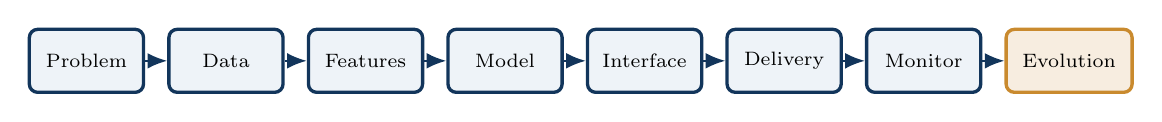
\begin{tikzpicture}[node distance=0.28cm]
  \node[flowbox, minimum width=1.45cm, minimum height=0.8cm] (problem) {\scriptsize Problem};
  \node[flowbox, minimum width=1.45cm, minimum height=0.8cm, right=of problem] (data) {\scriptsize Data};
  \node[flowbox, minimum width=1.45cm, minimum height=0.8cm, right=of data] (features) {\scriptsize Features};
  \node[flowbox, minimum width=1.45cm, minimum height=0.8cm, right=of features] (model) {\scriptsize Model};
  \node[flowbox, minimum width=1.45cm, minimum height=0.8cm, right=of model] (interface) {\scriptsize Interface};
  \node[flowbox, minimum width=1.45cm, minimum height=0.8cm, right=of interface] (delivery) {\scriptsize Delivery};
  \node[flowbox, minimum width=1.45cm, minimum height=0.8cm, right=of delivery] (monitor) {\scriptsize Monitor};
  \node[accentbox, minimum width=1.6cm, minimum height=0.8cm, right=of monitor] (evolution) {\scriptsize Evolution};
  \foreach \a/\b in {problem/data,data/features,features/model,model/interface,interface/delivery,delivery/monitor,monitor/evolution} {
    \draw[arrow] (\a) -- (\b);
  }
  \end{tikzpicture}

  \vspace{0.5em}
  \begin{block}{Today in the course}
  \textbf{Focus:} #1

  \textbf{Bridge:} #2
  \end{block}

  \begin{columns}[T]
  \column{0.48\textwidth}
  \begin{block}{Fraud case}
  {\footnotesize #3}
  \end{block}
  \column{0.48\textwidth}
  \begin{block}{Pasteurization case}
  {\footnotesize #4}
  \end{block}
  \end{columns}

  \vspace{0.3em}
  {\footnotesize \textbf{Course thread:} #5}
  \coursefooter
  \end{frame}
}

\newcommand{\classclosingframe}[4]{
  \begin{frame}{From This Class to the Next}
  \begin{block}{What stays with us}
  #1
  \end{block}

  \begin{columns}[T]
  \column{0.48\textwidth}
  \begin{block}{Project use}
  {\footnotesize #2}
  \end{block}
  \column{0.48\textwidth}
  \begin{block}{Next connection}
  {\footnotesize #3}
  \end{block}
  \end{columns}

  \vspace{0.3em}
  {\footnotesize \textbf{Course thread:} #4}
  \coursefooter
  \end{frame}
}

\tikzset{
  flowbox/.style={
    rounded corners=3pt,
    draw=courseblue,
    fill=courseice,
    very thick,
    minimum width=2.2cm,
    minimum height=0.9cm,
    align=center,
    font=\small
  },
  accentbox/.style={
    rounded corners=3pt,
    draw=coursegold,
    fill=coursegold!15,
    very thick,
    minimum width=2.2cm,
    minimum height=0.9cm,
    align=center,
    font=\small
  },
  arrow/.style={
    -{Latex[length=2.5mm,width=2mm]},
    thick,
    draw=courseblue
  }
}


\title{Class 7: Functions and Good Practices}
\author{\coursename}
\date{}

\begin{document}

\frame{\titlepage \coursefooter}

\begin{frame}{Agenda}
\begin{itemize}
\item Writing small, single-purpose functions.
\item Multiple return values, and functions as values themselves.
\item Splitting code across files: modules, \texttt{import} versus \texttt{from...import}.
\item The Zen of Python and what ``good practice'' means in this course.
\item Naming, readability, refactoring, and a first taste of testing.
\end{itemize}
\coursefooter
\end{frame}

\begin{frame}{Learning goals}
\learninggoals{
\begin{itemize}
\item Write functions with clear inputs, outputs, and a single responsibility.
\item Return and unpack multiple values from one function.
\item Organize functions into a module and import them elsewhere.
\item Apply naming and structure conventions that make code easier to read and change.
\item Recognize refactoring opportunities and describe a function's behavior precisely enough to test it.
\end{itemize}
}
\coursefooter
\end{frame}

\coursecontextframe
{Functions as the unit of reuse, and the habits that keep a growing codebase readable.}
{Class 4 introduced \texttt{def}; this class asks what makes a function --- and the file around it --- genuinely good.}
{The fraud model's training script and API are each only a handful of functions; their clarity is what makes the pipeline trustworthy.}
{The pasteurization simulator, `pasteurization/synth\_sensors.py`, is built almost entirely from small, typed, single-purpose functions --- our main case study today.}
{Good functions are what let a one-person script become a codebase other people, including future you, can safely change.}

\begin{frame}[fragile]{Small, single-purpose functions}
\begin{lstlisting}[style=coursepython]
def ramp(start: float, end: float, n: int) -> np.ndarray:
    return np.linspace(start, end, n)

def smooth_noise(n: int, scale: float) -> np.ndarray:
    steps = rng.normal(0, scale, size=n)
    return np.cumsum(steps) / max(n, 1)

def mu_of_T(T: np.ndarray) -> np.ndarray:
    return np.interp(T, [10, 72], [VISC_COLD, VISC_HOT])
\end{lstlisting}
\begin{itemize}
\item From `pasteurization/synth\_sensors.py`: each function does exactly one thing and says so in its name and type hints.
\item Type hints (\texttt{start: float}, \texttt{-> np.ndarray}) are optional in Python but document intent for free.
\end{itemize}
\coursefooter
\end{frame}

\begin{frame}[fragile]{Multiple return values}
\begin{lstlisting}[style=coursepython]
def simulate_batch(bid, start_time=0.0):
    ...
    return df, t

df, t = simulate_batch(BATCH_ID)
\end{lstlisting}
\begin{itemize}
\item Python functions can return several values at once, packed as a tuple and unpacked on the caller's side.
\item `simulate_batch` in `synth\_sensors.py` returns both the simulated batch (\texttt{df}) and the elapsed time (\texttt{t}) --- both needed by the caller, neither deserving its own function.
\end{itemize}
\coursefooter
\end{frame}

\begin{frame}[fragile]{Functions as values}
\begin{lstlisting}[style=coursepython]
SEGMENT_FUNCS = {
    "Idle": seg_idle,
    "Fill": seg_fill,
    "HeatUp": seg_heatup,
    "Hold": seg_hold,
    "Cool": seg_cool,
    "Discharge": seg_discharge,
}
\end{lstlisting}
\begin{itemize}
\item From `pasteurization/serving.py`: a dictionary whose values are functions, not numbers or strings.
\item This replaces a long \texttt{if}/\texttt{elif} chain with a single lookup --- functions are ordinary values in Python, storable and passable like anything else.
\end{itemize}
\coursefooter
\end{frame}

\begin{frame}[fragile]{Splitting code into modules}
\begin{lstlisting}[style=coursepython]
# pasteurization/serving.py
from synth_sensors import (
    seg_idle, seg_fill, seg_heatup, seg_hold, seg_cool, seg_discharge,
    PROD_RANGES, DT, rng, mu_of_T
)
\end{lstlisting}
\begin{itemize}
\item `synth\_sensors.py` is a module: a file of related functions and constants that other files import from.
\item \texttt{import x} loads the whole module under one name; \texttt{from x import a, b} pulls specific names directly into scope.
\item As a script grows, moving related functions into their own file is usually the first real refactor a project needs.
\end{itemize}
\coursefooter
\end{frame}

\begin{frame}{Good practice: what it is, and why it evolved}
\begin{itemize}
\item Best practices come from decades of programmer experience, not arbitrary style preference.
\item They increase productivity and decrease the mental overhead of reading someone else's code --- including your own, months later.
\item Python encodes much of its own philosophy in the Zen of Python (\texttt{import this}).
\end{itemize}
\coursefooter
\end{frame}

\begin{frame}{The Zen of Python, selected}
\begin{itemize}
\item ``Explicit is better than implicit.''
\item ``Readability counts.''
\item ``Simple is better than complex.''
\item ``Errors should never pass silently. Unless explicitly silenced.''
\item ``In the face of ambiguity, refuse the temptation to guess.''
\end{itemize}
\begin{block}{Course translation}
Every one of these lines is really an argument for naming things clearly, handling failure on purpose, and not being clever for its own sake.
\end{block}
\coursefooter
\end{frame}

\begin{frame}{Naming conventions}
\begin{tabularx}{\textwidth}{>{\bfseries}l X}
Style & Used for \\
\toprule
\texttt{snake\_case} & Ordinary variables and function names, e.g.\ \texttt{smooth\_noise}. \\
\texttt{UPPER\_CASE} & Module-level constants, e.g.\ \texttt{N\_BATCHES}, \texttt{MODEL\_ACCURACY}. \\
\texttt{PascalCase} & Class names, e.g.\ \texttt{RandomForestClassifier}, \texttt{StandardScaler}. \\
Leading \texttt{\_} & A hint that a name is private or internal to a module. \\
\bottomrule
\end{tabularx}
\vspace{0.4em}
\begin{itemize}
\item Every one of these examples already exists somewhere in this repository --- the convention is not just theory.
\end{itemize}
\coursefooter
\end{frame}

\begin{frame}{Refactoring: guard clauses}
\begin{columns}[T]
\column{0.48\textwidth}
\textbf{Deeply nested}
\begin{itemize}
\item \texttt{if} data is valid:
\begin{itemize}
\item \texttt{if} model is loaded:
\begin{itemize}
\item run prediction
\end{itemize}
\end{itemize}
\end{itemize}
\column{0.48\textwidth}
\textbf{Guard clauses}
\begin{itemize}
\item \texttt{if not} valid: \texttt{return}
\item \texttt{if not} loaded: \texttt{return}
\item run prediction
\end{itemize}
\end{columns}
\vspace{0.5em}
\begin{block}{Idea}
Handle the exceptional case first and return early, so the main logic is not buried three levels deep.
\end{block}
\coursefooter
\end{frame}

\begin{frame}{Readability and comments}
\begin{itemize}
\item Use \texttt{enumerate()} instead of a manual counter when you need both index and value.
\item Comments should explain \emph{why}, not restate \emph{what} the code already says.
\item Keep comments up to date --- an outdated comment is worse than no comment.
\item Prefer a well-named variable over a comment explaining a badly-named one.
\end{itemize}
\coursefooter
\end{frame}

\begin{frame}[fragile]{A first taste of testing}
\begin{lstlisting}[style=coursepython]
def ramp(start: float, end: float, n: int) -> np.ndarray:
    return np.linspace(start, end, n)

assert list(ramp(0.0, 10.0, 2)) == [0.0, 10.0]
\end{lstlisting}
\begin{itemize}
\item Black-box testing means checking a function's output for known inputs, without caring how it is implemented inside.
\item A single-purpose, typed function like \texttt{ramp} is exactly the kind of function that is easy to test this way.
\item Class 11 formalizes this idea further once scikit-learn's own API enters the picture.
\end{itemize}
\coursefooter
\end{frame}

\begin{frame}{How the repo already uses today's building blocks}
\repoactivity{
\begin{itemize}
\item `pasteurization/synth\_sensors.py` is a full module of small, typed, single-purpose functions --- read it end to end as a worked example of today's lecture.
\item `pasteurization/serving.py` imports selectively from that module and stores functions inside a dictionary.
\item Pick one function from `synth\_sensors.py` and rewrite its one-line docstring in your own words.
\end{itemize}
}
\coursefooter
\end{frame}

\begin{frame}{Discussion prompt}
\begin{block}{Question}
`SEGMENT_FUNCS` replaces an \texttt{if}/\texttt{elif} chain with a dictionary lookup. What would you lose, if anything, by keeping the \texttt{if}/\texttt{elif} chain instead?
\end{block}
\begin{itemize}
\item Encourages weighing readability and extensibility against a construct students may find less familiar than the alternative.
\end{itemize}
\coursefooter
\end{frame}

\begin{frame}{Papers and materials}
\readinglist{
Sommerville, \textit{Software Engineering};\
Chip Huyen, \textit{Designing Machine Learning Systems};\
\href{https://scikit-learn.org/stable/}{scikit-learn documentation}.
}
\coursefooter
\end{frame}

\classclosingframe
{\begin{itemize}
\item A good function is small, named clearly, and returns exactly what its caller needs --- one value or several.
\item Modules let related functions live together and be imported where needed.
\item Naming, guard clauses, and small testable functions are habits, not one-time decisions.
\end{itemize}}
{Before your project script passes 50 lines, check whether it should already be split into functions, and those functions into a module.}
{Class 8 goes one level further: bundling functions and the data they operate on together, inside a class.}
{Functions group behavior; next class groups behavior with the data it belongs to.}

\end{document}
